% Latex对控制序列的大小写很敏感
%-*- coding: UTF-8 -*-

% LATEX命令格式:
	% 无参数:\command
	% 有n个参数:\command{<arg1><arg2>...<argn>}
	% 有可选参数:\command[<arg>]{<arg1><arg2>...<argn>}
\documentclass[UTF8]{ctexart}  %这样写可以解析中文,包含一个可选参数
% 这里是注释
\title{\heiti 杂谈勾股定理}
\author{\kaishu 刘海燕}
\date{\today}
% 上面三行信息并不会马上出现在编译的结果中,而是要通过第11行的\maketitle进行排版
\newtheorem{thm}{定理}
\newcommand\degree{^\circ}
\usepackage{graphicx} % 插图功能是由graphicx宏包提供的
\usepackage{float}
\usepackage{geometry} %设计页面尺寸
\geometry{a6paper,centering,scale=0.8}
\usepackage[format=hang,font=small,textfont=it]{caption} %改变图表标题的格式
%\usepackage[nottoc]{tocbibind}
\bibliographystyle{plain} % 声明参考文献的格式

% 以上在\begin{document}字段之前的部分称为 导言区。导言区通常用来对文档的性质做一些设置或者自定义一些命令。
\begin{document}
	% 论文的正文部分,也就是直接输出的部分
	% 所有目录、编号和页码都是自动生成的
	\maketitle
	
	%%%% 摘要
	\begin{abstract}
		这是一篇关于勾股定理的小短文。
	\end{abstract}
	%%%% 摘要
	
	\tableofcontents % 输出目录
	
	\section{勾股定理在古代} % 设置新的一节
	% 段前不需要打空格,TEX会自动完成文字的缩进。即使段前打了空格,TEX也会将其忽略。
	% 空格使用----通常汉字后的空格会被忽略,而其他符号后的空格则保留。所以,可以使用单个换行来代表空格。
	% 脚注----\footnote{text}
	% 改变字体,表示强调(emphasis):\emph{text}
	西方勾股定理为毕达哥拉斯定理,将勾股定理的发现归功于公元前
	6
	世纪的毕达哥拉斯学派。该学派得到了一个法则,可以求出排成直角三角形三边的三元数组。毕达哥拉斯学派没有书面著作,该定理的严格表述和证明则见于欧几里得\footnote{欧几里得,约公元前330--275年。}《几何原本》的命题
	47:“直角三角形斜边上的正方形\emph{等于}两直角边上的两个正方形之和。”证明是用面积做的。
	
	% 换行使用----空行起分段作用,但是多个空行并没有过多的作用。
	% quote环境将内容单独分行,增加缩进和上下间距排印,以突出引用的部分。随后在内容里使用\zihao{-5}\kaishu更换字体,以达到引用的效果,-5表示小五号。
	% \zihao与\kaishu命令会影响后面所有的文字,直至整个分组结束。一个LATEX环境就是一个分组,所以这两个命令会影响整个quote环境。
	% 
	我国《周髀算经》载商高(约公元前 12 世纪)答周公问:
	\begin{quote}
		勾广三,股修四,径隅五。
	\end{quote}
	又载陈子\footnote{陈子,约公元前7---6世纪}答荣方问:
	\begin{quote}
		\zihao{-5}\kaishu 若求邪至日者,以日下为勾,日高为股,勾股各自乘,并而开方除之,得邪至日。
	\end{quote}
	都较古希腊更早。后者已经明确道出勾股定理的一 般形式。图是我国古代对勾股定理的一种证明。
	
	%%%% 插图
	% width设置图形在文档中显示的宽度,还有一些参数scale=放缩因子、height=高度 等
	% 20191004097.jpg是图片的文件名(放在源文件所在的目录中)
	% 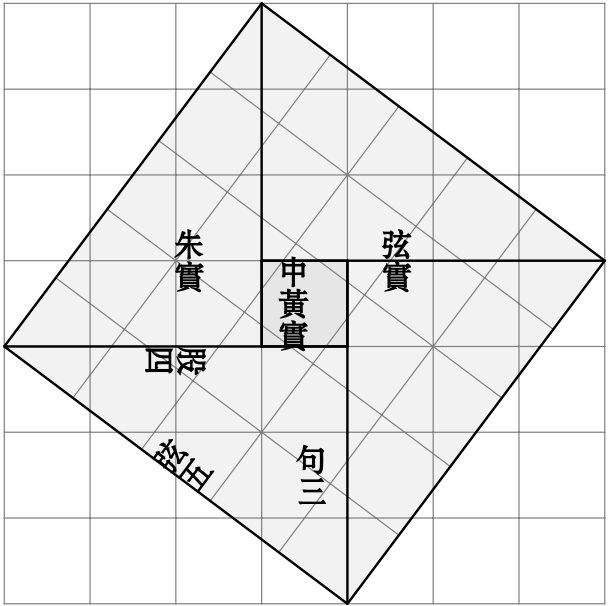
\includegraphics[width=3cm]{gougu.png}
	
	% 插入的图形就是一个有内容的矩形盒子,在正文中和一个很大的字符没有多少区别。因此会与文本混在一起。
	% 所以,通常把图形放在一个可以变动的相对位置的环境中,称为浮动体,放在figure环境中。
	% 可选参数ht表示浮动体可以出现在环境周围的文本所在处(here)和一页的顶部(top)
	% \label命令给图像定义一个标签,使用这个标签就可以在文章的其他地方引用图像。
	\begin{figure}[ht]
		\centering
		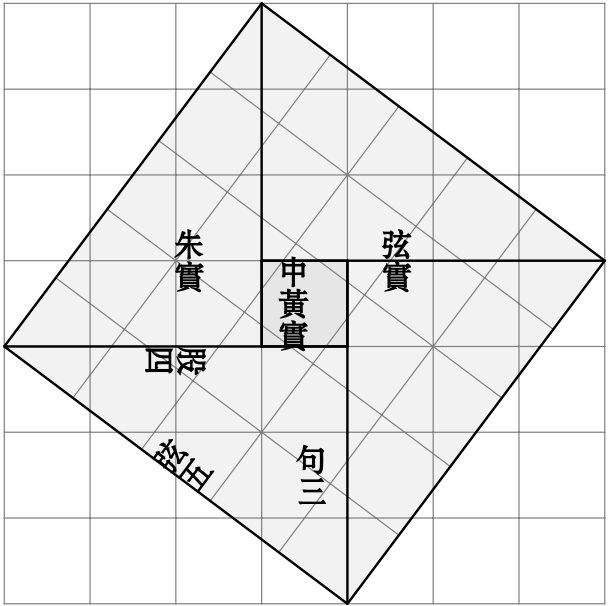
\includegraphics[scale=0.4]{gougu.png}
		\caption {宋赵爽在《周髀算经》注中作的弦图(仿制),该图给出了勾股定 理的一个极具对称美的证明。}
		\label{fig:20191004097}
	\end{figure}
	%%%% 插图
	
	
	\section{勾股定理的近代形式}
	\begin{thm}[勾股定理]
		直角三角形斜边的平方等于两腰的平方和。
		
		可以用符号语言表述为:设直角三角形$ABC$,其中$\angle C=90^\circ$,$90\degree$则有
		%%%% 公式
		\begin{equation}
			AB^2=BC^2+AC^2
		\end{equation}
		%%%% 公式
	\end{thm}
	满足式(1)的整数称为勾股数。第1节所说毕达哥拉斯学派得到的三元数组就是勾股数。下表列出一些较小的勾股数:
	%%%% 表格
	% |rrr|表示表格有3列,都是右对齐,第一列前面和第三列后面各有一条垂直的表格线
	% 在环境内部,行与行之间用命令\\隔开,每行内部的表项使用&隔开
	% 表中的横线是用\hline命令产生的
	% 表格和插图一样,都是一个比较大的盒子,一般也是放在浮动环境中,即table环境
	% [H]表示让表格固定位置
	\begin{table}[H]
		\begin{tabular}{|rrr|}
			\hline
			直角边$a$ & 直角边$b$ & 斜边$c$\\
			\hline
			3 & 4 & 5\\
			5 & 12 & 13\\
			\hline
		\end{tabular}
		\quad %产生长为2em的空白
		($a^2+b^2=c^2$)
	\end{table}
	%%%% 表格
	
	\bibliography{math} %提示TEX从文献数据库math中获取文献信息,打印参考文献列表。
\end{document}